\chapter{Introduction}
\label{ch:introduction}

% ---------------------------------------------------------------------
%  This is a WORKED-EXAMPLE chapter. Read the % comments to learn the
%  LaTeX patterns, then replace the body text with your own writing.
%  Paragraphs are separated by a blank line; single line breaks in the
%  source are ignored.
% ---------------------------------------------------------------------

This thesis investigates \textbf{<your research topic>}. The opening of an
introduction sets the scene: what is the broad area, why does it matter, and
what gap does your work address? \lipsum[1]

% --- Citations -------------------------------------------------------
% natbib provides two main citation commands:
%   \citet{key}  ->  "Smith (2020)"    (author is part of the sentence)
%   \citep{key}  ->  "(Smith, 2020)"   (fully parenthetical)
% Cite several sources at once with a comma: \citep{a,b,c}.
Foundational background is provided by \citet{bridson2015}. Several authors have
studied closely related problems \citep{smith2020, lee2019}, and practical
guidance is also available online \citep{example2024}.

% --- Referring to a figure -------------------------------------------
% Put \label{fig:...} inside the figure, then refer to it with
% \ref{fig:...}. Use a non-breaking space (~) before \ref so the number
% never starts a new line. Never hard-code "Figure 1".
Figure~\ref{fig:intro-example} shows a placeholder image; replace it with one of
your own.

\begin{figure}[h]
    \centering
    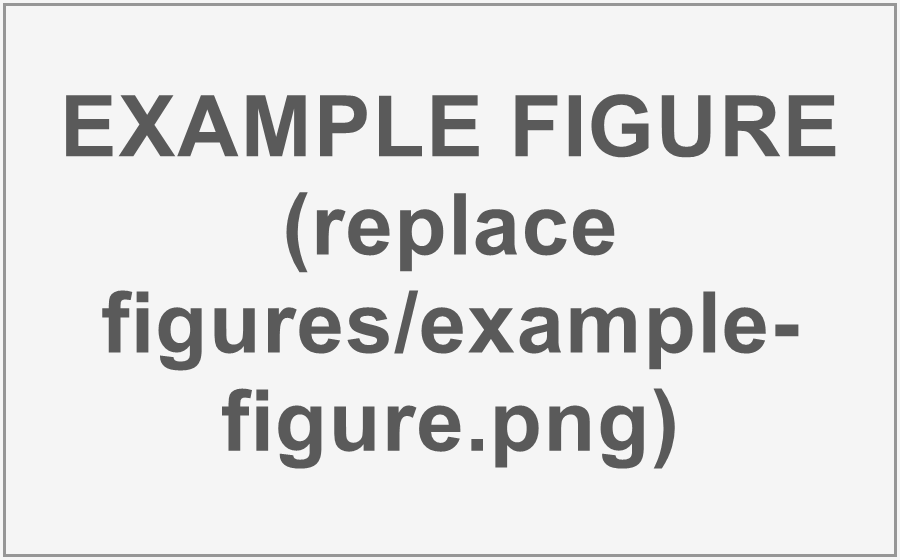
\includegraphics[width=0.6\linewidth]{figures/example-figure.png}
    \caption{A placeholder figure. A good caption explains what the reader is
             looking at and why it matters. Replace the image in
             \texttt{figures/} with your own.}
    \label{fig:intro-example}
\end{figure}

\section{Background and Motivation}
\label{sec:motivation}
\lipsum[2]

\section{Contributions}
\label{sec:contributions}

% An ordered list (enumerate). Use itemize instead for bullet points.
The main contributions of this thesis are:
\begin{enumerate}
    \item The first contribution, stated as a single clear sentence.
    \item The second contribution, which builds on the first.
    \item The third contribution and why it matters.
\end{enumerate}

\section{Thesis Outline}
\label{sec:outline}

% \paragraph{} creates a bold run-in heading -- handy for an outline.
% Note how Chapter~\ref{ch:introduction} cross-references this chapter
% by its \label, so the numbering stays correct if chapters move.
\paragraph{Chapter~\ref{ch:introduction}.} Introduces the problem, motivation, and contributions.

\paragraph{Chapter~\ref{ch:background}.} Reviews the relevant background and related work.

\paragraph{Chapter~\ref{ch:methodology}.} Describes the methodology and experimental setup.

\paragraph{Chapter~\ref{ch:results}.} Presents and analyses the results.

\paragraph{Chapter~\ref{ch:discussion}.} Discusses the findings, limitations, and implications.

\paragraph{Chapter~\ref{ch:conclusion}.} Concludes and outlines directions for future work.
